\documentclass[10pt,twocolumn,journal]{IEEEtran}
% XeLaTeX: all fonts are resolved from the local installation.
\usepackage{fontspec}
\defaultfontfeatures{Ligatures=TeX}
\setmainfont[
  BoldFont=TeXGyreTermes-Bold,
  ItalicFont=TeXGyreTermes-Italic,
  BoldItalicFont=TeXGyreTermes-BoldItalic,
  SmallCapsFont=TeXGyreTermes-Regular,
  SmallCapsFeatures={Letters=SmallCaps}
]{TeXGyreTermes-Regular}
\IfFontExistsTF{Arial}{\setsansfont{Arial}}{\setsansfont{Liberation Sans}}
\setmonofont{TeXGyreCursor-Regular}

\usepackage[margin=1in,bottom=1.12in]{geometry}
\usepackage{xeCJK}
% Build script resolves installed standalone Chinese font files.
% The generated file contains local font paths only; no font binaries are distributed.
\InputIfFileExists{../font_local_zh.tex}{}{%
  \setCJKmainfont[BoldFont=FandolSong-Bold.otf,ItalicFont=FandolKai-Regular.otf,SmallCapsFont=FandolSong-Regular.otf]{FandolSong-Regular.otf}
  \setCJKsansfont[BoldFont=FandolHei-Bold.otf]{FandolHei-Regular.otf}
  \setCJKmonofont{FandolFang-Regular.otf}
}

\usepackage{amsmath,amssymb}
\usepackage{booktabs,array,multirow}
\usepackage{graphicx}
\usepackage{xurl}
\usepackage{xr-hyper}
\usepackage[hidelinks,unicode]{hyperref}
\urlstyle{same}
\usepackage{fancyhdr}
\usepackage{flushend}
\externaldocument{supplement}[supplement.pdf]
\graphicspath{{figures/}}
\setlength{\emergencystretch}{4em}
\renewcommand{\figurename}{图}
\renewcommand{\tablename}{表}
\renewcommand{\refname}{参考文献}
\renewcommand{\abstractname}{摘要}
\renewcommand{\IEEEkeywordsname}{关键词}
\DeclareMathOperator{\NLL}{NLL}
\DeclareMathOperator{\CRPS}{CRPS}
\DeclareMathOperator{\Std}{std}
\pagestyle{fancy}
\fancyhf{}
\fancyhead[L]{\scriptsize BELOW ZERO}
\fancyhead[R]{\scriptsize\thepage}
\renewcommand{\headrulewidth}{0pt}
\hypersetup{pdftitle={Below Zero：面向下限删失 RAW 图像的空间自适应条件读出抽样},pdfauthor={},pdfsubject={中文学术译稿；与最终英文编辑稿对应}}
\newcommand{\BZAuthorBlockEN}{Yaogeng Jiang\\Independent Researcher\\\href{mailto:y.g.jiang@sjtu.edu.cn}{y.g.jiang@sjtu.edu.cn}}
\newcommand{\BZAuthorBlockZH}{姜尧耕\\独立研究者\\\href{mailto:y.g.jiang@sjtu.edu.cn}{y.g.jiang@sjtu.edu.cn}}
\newcommand{\BZPDFAuthors}{Yaogeng Jiang}

\hypersetup{pdfauthor={\BZPDFAuthors}}
\begin{document}
\title{{\normalsize \href{https://github.com/y-g-jiang/Video-RAW-Black-Level-Correction-Net/tree/main/below_zero}{代码与数据}}\\[6pt]Below Zero：面向下限删失 RAW 图像的\\空间自适应条件读出抽样}
\author{\BZAuthorBlockZH}
\maketitle
\thispagestyle{fancy}

\begin{abstract}
将黑电平扣除后的 RAW 测量值钳位到零，会丢弃负读出码并改变暗部统计。本文提出一种单帧补全方法，在保留每个正测量值的同时，于删失位置抽样有符号整数。多尺度卷积估计器预测局部信号，经校准的量化 Poisson--Gaussian 解码器再将每次预测转换为零及负码的概率。对补全 Bayer 图像重新钳位即可精确复现输入。在经校准的高增益传感器模型下，N0/PG 在 138 幅留出源图像上，相对于局部似然估计将超额 Kullback--Leibler 散度从 0.001723 降至 0.000313 nats，实际观测码值的负对数似然每个删失码降低 0.001407 nats；每幅源图像的 KL 均有改善。区域分析表明，经典估计器在近黑区域已很准确，而较大差距出现在较高信号和非均匀邻域。在保持预测分布集合不变的条件下置换其位置，误差仍会增大，表明空间分配很重要。两次保留有符号参考值的真实曝光显示，神经与局部条件抽样均能恢复去马赛克暗部起伏。这些结果建立了一种测量保持的下限删失 RAW 补全方法，并量化了学习式空间估计对条件读出精度的贡献。
\end{abstract}

\begin{IEEEkeywords}
计算成像，删失测量，Bayer RAW 图像，Poisson--Gaussian 噪声，概率重建，去马赛克。
\end{IEEEkeywords}

\section{引言与相关工作}
黑电平扣除使 RAW 传感器测量值围绕一个有符号原点分布。即使光学信号非负，读出噪声也会在暗区产生负码。将这些码钳位到零会改变观测噪声的均值和变异性 \cite{foi2008,foi2009}，并可能影响后续插值和平均。下限钳位见于有文档记录的相机处理管线 \cite{mathworksISP}、相机文件调查 \cite{librawD5300,claffReadNoise}，以及 AIM 2025 RAW 视频挑战中 VMCL-ISP 团队报告的负噪声钳位 \cite{aim2025Video}。RAW 图像评价接口也会施加非负输出约束 \cite{sonyAIM2025}。

本文的任务是根据单张下限删失 Bayer 图像补全合理的有符号读出样本。零观测合并了原始量化零码与被钳位移除的任意负整数。补全必须填充这些位置，同时保持所有正测量值不变，从而保留后续处理所用的传感器测量表示。

关键困难在于：同样的零观测未必对应同样的条件分布。受照边缘旁的零码与均匀暗区内的零码，对被隐藏的读出具有不同含义。附近仍为正的测量值携带了这种差异，而局部恒定信号模型容易将其平滑掉。估计空间变化的信号场之后，同一个物理解码器便可为不同位置赋予不同的读出概率分布。

N0/PG 将空间估计与条件解码分离。NAF 风格卷积网络 \cite{nafnet} 根据打包 Bayer 图像和校准参数预测非负信号场，量化 Poisson--Gaussian（PG）解码器再计算给定零观测时原始整数码的条件分布。采样器仅填充删失像素，恒等分支复制每个正码（图~\ref{fig:pipeline}）。

\begin{figure*}[t]
\centering
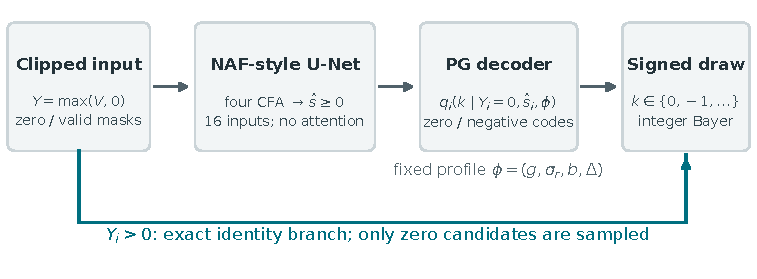
\includegraphics[width=\textwidth]{f01_pipeline.pdf}
\caption{空间自适应有符号 RAW 补全。网络为量化 PG 解码器预测局部信号参数。从零观测对应的非正整数分布中抽样；已观测正码经恒等分支原样通过。}
\label{fig:pipeline}
\end{figure*}

本文进一步考察：空间上下文能否比局部噪声模型拟合更准确地估计条件读出分布？我们通过 138 幅留出源图评价分布精度，分析收益与信号、邻域结构的关系，并将补全的有符号样本用于去马赛克和固定颜色渲染。

\subsection{相关工作}
\subsubsection{删失测量与 RAW 噪声模型}
条件插补是处理删失观测的标准方法。在 Tobit 回归中，O'Neill \cite{oneill2024} 采用潜在数据增强，保留未删失响应，并从其条件分布中抽取删失响应。在成像领域，Kodgirwar 等人 \cite{kodgirwar2024} 为多曝光叠层成像融合推断饱和 Poisson 计数。本文场景则将条件读出补全应用于具有量化 PG 噪声的单张 Bayer 图像，同时保留实测正码和原始零码的离散概率。

Foi 等人 \cite{foi2008} 建立了包含钳位的实用 RAW 噪声 PG 模型。随后，Foi \cite{foi2009} 推导了变换和逆校正，使钳位异方差观测的去噪成为可能。其统计模型构成本文条件解码器的基础。本文输出为删失像素处抽样的整数读出，而其去噪目标是估计潜在信号。Foi-qPG 比较方法先应用这些变换/滤波思想，再使用与其他估计器相同的量化条件解码（第~\ref{sec:baselines} 节）。

物理 RAW 噪声还包含独立 Gaussian 读出噪声之外的效应。Wei 等人 \cite{wei2020} 建模了极弱光成像的传感器噪声分量，Zhang 等人 \cite{zhang2021} 讨论相关噪声与量化，Mohammadi 等人 \cite{mohammadi2026} 研究黑电平偏差。即使保留的零码和正码不变，这些效应仍可能改变已丢失负码的条件分布。

\subsubsection{学习式估计与条件抽样}
NAFNet \cite{nafnet} 为图像恢复提供了高效的卷积模块。本文使用独立实现的 NAF 风格编码器—解码器，不含池化通道调制，因此估计器具有有限空间依赖。其输出是以 DN 表示的信号参数；经校准的 PG 模型决定相应概率。

学习先验与测量模型已被结合用于深度平衡重建 \cite{gilton2021}、凸正则化 \cite{goujon2023} 和生成先验 Bayesian 反演 \cite{bohra2022}。这些方法推断潜在图像；本文所求则是给定零观测时被丢弃的整数读出。Gnanasambandam 等人的 Poisson 反卷积研究 \cite{gnanasambandam2024} 启发我们考察空间估计选择的影响，并用恰当概率评分 \cite{gneiting2007} 衡量所得条件分布。

\subsubsection{去马赛克与下游处理}
联合去马赛克与去噪利用空间和颜色相关性恢复干净图像 \cite{gharbi2016}。本文的任务发生在更靠前的处理环节：在插值之前补全合理的有符号测量。为考察其影响，我们使用自适应同质性导向（AHD）去马赛克 \cite{hirakawa2005}，并指定 LibRaw 实现 \cite{libraw}。

\section{条件读出补全}
\subsection{量化的下限删失读出}
令 $s_i\geq0$ 为以数字单位（DN）表示的期望光学信号，$g$ 为转换增益，单位为 DN/电子，$b_i$ 为相对标称黑电平的已知偏移。在校准 PG 模型下，光子计数与连续有符号读出满足
\begin{align}
N_i&\sim\operatorname{Poisson}(s_i/g),\label{eq:pois}\\
Z_i&=gN_i+b_i+\epsilon_i,\qquad \epsilon_i\sim\mathcal N(0,\sigma_r^2).\label{eq:forward}
\end{align}
以 1 DN 为步长作最近整数量化，得到 $V_i=\lfloor Z_i+1/2\rfloor$。选择共同的有符号码原点后，本文将下限写为零；文件域中位于其他码值的下限可通过平移该原点表示。下限删失随后产生
\begin{equation}
Y_i=\max(V_i,0),\qquad \mathcal Z=\{i:Y_i=0\}.\label{eq:censor}
\end{equation}
模拟器包含 $16383-512=15871$ DN 的上限饱和。所评价的样本保持在 ADC 物理下界之上；在这一范围内，本文采用无界 Gaussian 读出噪声模型。

对于 $k\leq0$，定义量化码值的概率质量
\begin{align}
a_k(s,b)=\sum_{n=0}^{\infty}\operatorname{Pois}(n;s/g)
\bigg[&\Phi\!\left(\frac{k+1/2-gn-b}{\sigma_r}\right)\nonumber\\[-2pt]
-&\Phi\!\left(\frac{k-1/2-gn-b}{\sigma_r}\right)\bigg],\label{eq:bin}
\end{align}
其中 $\Phi$ 为标准正态累积分布函数。零观测概率为
\begin{equation}
c(s,b)=\sum_{n=0}^{\infty}\operatorname{Pois}(n;s/g)
\Phi\!\left(\frac{1/2-gn-b}{\sigma_r}\right).\label{eq:zeroevent}
\end{equation}
$+1/2$ DN 边界同时包含原始零码的量化区间和所有负码区间。

给定信号估计 $\hat s_i$，解码器返回
\begin{equation}
q_i(k)=\frac{a_k(\hat s_i,b_i)}{c(\hat s_i,b_i)},\qquad k=0,-1,-2,\ldots.\label{eq:posterior}
\end{equation}
式~\eqref{eq:bin} 的区间积分保留了 $k=0$ 处的离散原子，式~\eqref{eq:posterior} 的归一化则以完整零观测事件为条件。图~\ref{fig:counterexamples} 展示了所得分布如何随图像位置变化。

\subsection{测量保持补全}
对每个零候选位置，从其预测条件分布中抽取 $K_i$，并构造
\begin{equation}
\widetilde V_i=\begin{cases}
Y_i,&Y_i>0,\\
K_i,\quad K_i\sim q_i,&Y_i=0.
\end{cases}\label{eq:output}
\end{equation}
恒等分支与 $q_i$ 的非正支撑保证 $\max(\widetilde V_i,0)=Y_i$ 精确成立。条件样本表达被隐藏的读出起伏，而不是干净信号的点估计；随机抽样与条件均值因而服务于不同损失。本文使用分布评分评价预测概率律，抽样与均值的风险恒等式见补充材料第 I 节。

模拟器利用真实 $s_i$ 提供已知信号参考
\begin{equation}
p^{\star}_i(k)=a_k(s_i,b_i)/c(s_i,b_i),\label{eq:oracle}
\end{equation}
推理时将信号场固定为 $\hat s_i$，$q_i$ 描述条件读出变化。在该估计场条件下，各像素抽样相互独立。

\section{学习空间自适应读出分布}
\subsection{信号估计器}
本文将 Bayer 相位打包为 $[R,G_1,G_2,B]$，输入变换后的测量图、零码指示图、已知偏移、有效性掩码和校准常量。有效性掩码区分填充与实测零码，偏移量同时输入估计器和 PG 解码器。

NAF 风格编码器—解码器通过加性跳跃连接和像素重排上采样融合四级下采样阶段的多尺度特征。逐像素归一化、逐通道卷积与乘性门构成有限空间依赖，不含全局池化或注意力。四通道 softplus 头预测以 DN 表示的 $\hat s_i\geq0$，解码器使用电子数均值 $\hat s_i/g$。模型有 10,913,380 个参数；补充材料第 II 节列出输入通道与各阶段维度。

\subsection{以条件分布为目标进行训练}
合成监督提供 $s_i$ 和条件目标 $p_i^\star$。本文在有效零候选上最小化交叉熵：
\begin{equation}
\mathcal L(\theta)=-\frac{1}{|\mathcal Z|}
\sum_{i\in\mathcal Z}\sum_{k\leq0}p^{\star}_i(k)\log q_{\theta,i}(k).
\label{eq:loss}
\end{equation}
实现在包含显式尾类别的有限类别表示上评价式~\eqref{eq:loss}。目标熵与网络无关，因此最小化该损失就是最小化相对于已知信号目标的散度。梯度经物理解码器传回估计器，使信号预测以条件分布精度为优化目标。合成潜在信号用于构造监督目标和评价参考。解码器接收已知校准参数及逐样本给定的偏移量，优化仅更新空间估计器。

\subsection{离散分布的数值计算与坐标索引抽样}
条件分布逐一表示 $0,-1,\ldots,-304$，并用一个类别表示 $V\leq-305$。计算似然和抽样时，尾类别会进一步分辨到单个整数码。补充材料第 III 节说明条件尾部分布的求值、数值误差界与坐标索引采样。



\begin{figure*}[t]
\centering
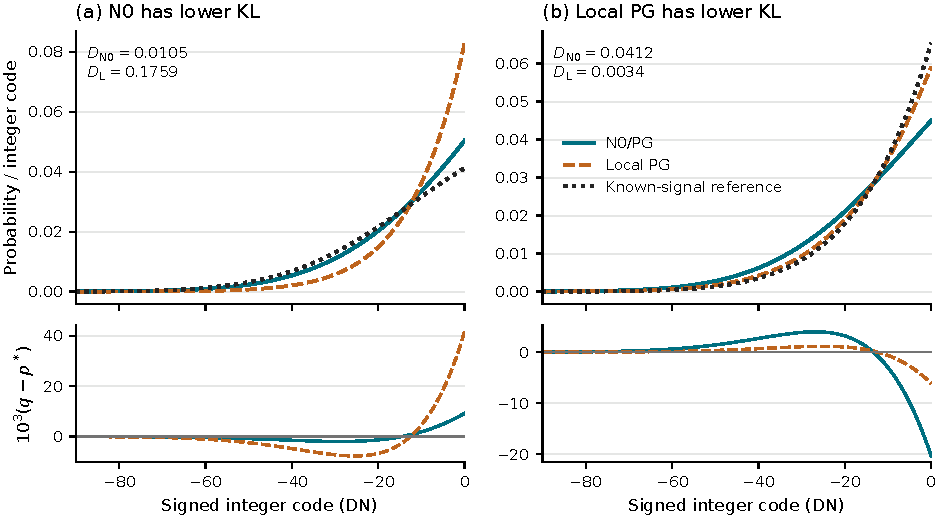
\includegraphics[width=\textwidth]{f02_pmf_counterexamples.pdf}
\caption{两个高梯度开发集位置的条件 PMF，均在评价后选取，用于展示两种方法在不同位置上各有优势的结果。上：N0/PG、Local PG 与已知信号分布。下：有符号概率误差。N0 在（a）中更准确，Local PG 在（b）中更准确。}
\label{fig:counterexamples}
\end{figure*}

\section{实验}
\subsection{数据、校准与训练}
实验采用 Panasonic S5 II ISO12800 的校准参数（表~\ref{tab:protocol}）。增益来自 JOT 测量 \cite{jot}，读出噪声由十幅暗帧的 R/$G_1$ 相位估计。合成信号、参考概率律及条件解码器使用同一 PG 模型，因此留出实验衡量的是匹配噪声假设下的空间条件分布估计；保留真实读出的案例则用于检验该模型在真实数据上的表现。

\begin{table}[t]
\centering\small
\caption{传感器校准参数与实验设置。}
\label{tab:protocol}
\begin{tabular}{@{}p{0.40\columnwidth}p{0.52\columnwidth}@{}}
\toprule
项目 & 设置\\
\midrule
传感器设置 & S5 II，ISO12800，机械快门，14 bit\\
增益 $g$ & 21.6010924121 DN/e$^{-}$\\
整数读出噪声 RMS & 24.9612744275 DN\\
模拟域 $\sigma_r$ & 24.9596051193 DN\\
标称黑电平 / 步长 & 512 DN / 1 DN\\
合成偏移 $b_c$ & 已知；均匀分布于 $[-0.25,0.25]$ DN\\
源图像划分 & 825 训练 / 137 开发 / 138 测试\\
训练 & Seed 7103；80,000 次更新\\
测试上下文 / 目标核心 & 128 和 256 / 中心 64 个打包像素\\
\bottomrule
\end{tabular}
\end{table}

合成信号场使用 DIV2K 和 BSDS500 的 1,100 幅彩色模板 \cite{div2k,bsds500}，划分为 825 幅训练、137 幅开发和 138 幅测试源图。训练样本中自然场景占 90\%，程序化控制占 10\%；曝光、颜色变化、量化与删失均按补充材料第 II 节所述 PG 生成过程完成。单次训练得到的 N0 模型依据开发集选取。

每幅留出源图生成两个曝光与噪声不同的场景，并分别在共享中心观测的 128 和 256 像素上下文中评价。138 幅源图共得到 552 个案例和 3,254,612 个评分条目；其中，256 像素上下文有 1,627,306 个不同候选位置。






\subsection{其他估计器}\label{sec:baselines}
Global PMF 对每个 CFA 相位使用由训练数据得到的平均条件分布。Global PG 则把训练得到的逐相位信号代入经校准的解码器。两者在测试时均给出空间恒定的预测。

Local PG 在同 CFA 的 $5\times5$ 邻域内，利用正码和零码删失事件的似然拟合信号。Local Bayes 在此基础上加入拟合的零点加 Gamma 先验，并对相应条件分布积分。两者使用开发集选定的同一邻域，中心观测只计一次。

Foi-qPG 基于 Foi 的钳位噪声变换 \cite{foi2009} 和 BM3D 滤波 \cite{bm3d} 构建，随后进行量化 PG 逆映射并使用共享的条件整数解码器。

N0 利用四个 CFA 相位估计多尺度信号场，主要局部基线则仅使用同 CFA 观测。开发集 Joint-CFA Bayes 对照也使用四相位，但保持局部恒定信号模型，用于检验在局部模型中加入跨相位观测能否缩小误差差距（补充材料第 VII-A 节）。

\subsection{评价准则}
对于每个保留作参考的有符号整数码 $v_i$，我们以负对数似然和离散秩概率评分评价预测的条件读出分布：
\begin{align}
\NLL(q_i,v_i)&=-\log q_i(v_i),\label{eq:nll}\\
\CRPS(q_i,v_i)&=\sum_{k\in\mathbb Z}
\left(F_{q_i}(k)-\mathbf{1}\{v_i\leq k\}\right)^2\Delta.\label{eq:crps}
\end{align}
NLL 以每候选项 nats 为单位，CRPS 以 DN 为单位，且 $\Delta=1$ DN。两者均按被隐藏的实际整数码值评分，尾类别内的码值也逐一计算。

模拟信号已知时，还可以用超额 KL 与累积分布差异直接比较预测条件分布和真实条件分布：
\begin{align}
D_i&=\sum_{k\leq0}p^{\star}_i(k)\log\frac{p^{\star}_i(k)}{q_i(k)},\label{eq:kl}\\
J_i&=\sum_{k\in\mathbb Z}\left(F_{q_i}(k)-F_{p^{\star}_i}(k)\right)^2\Delta.\label{eq:cdf}
\end{align}
超额 KL 和 $J_{\mathrm{CDF}}$ 使用共同的 306 类别表示，其中尾部合并为一类。NLL 与 CRPS 则分辨尾部内的各个码值。补充材料第 III 节给出相应数值界。

各评分先在源图内汇总，再对源图等权平均。成对源图 bootstrap 将同源的相关案例一起重采样；对 Local Bayes 和 Foi-qPG 的两项主要 KL 比较采用 97.5\% 区间。具体汇总方法与次要比较见补充材料第~\ref{sec:scoreaggregation}、\ref{sec:regionaldefinitions} 节。

\subsection{留出数据上的条件分布精度}
N0/PG 在所评价方法中取得最低的超额 KL、$J_{\mathrm{CDF}}$、NLL 和 CRPS（表~\ref{tab:holdout}）。已知信号概率律给出模拟器内可达到的参考水平，而零填充无法为被丢弃的负码赋予非零概率。

\begin{table*}[t]
\centering\small
\caption{138 幅留出源图上的条件分布评分；每幅源图含四个相关案例/上下文组合。评分采用源图等权。超额 KL 与 $J_{\mathrm{CDF}}$ 使用 306 类别；NLL 与 CRPS 分辨整数尾部。粗体表示最佳可部署方法。零填充对负标签赋予零概率，因此 KL/NLL 为无穷大；已知信号参考使用实际不可得的真实信号。}
\label{tab:holdout}
\begin{tabular}{@{}llrrrr@{}}
\toprule
方法 & 可用空间信息 & $10^3D_{\mathrm{KL}}\downarrow$ & NLL$\downarrow$ & CRPS$\downarrow$ & $10^3J_{\mathrm{CDF}}\downarrow$\\
\midrule
零填充 & 无 & $\infty$ & $\infty$ & 18.691235 & 10611.0233\\
Global PMF & 逐 CFA 训练分布律 & 3.4350 & 3.914828 & 8.112251 & 29.6469\\
Global PG & 逐 CFA 训练信号 & 3.3399 & 3.914723 & 8.111302 & 28.7879\\
Local PG & 同 CFA $5\times5$ & 1.7228 & 3.912975 & 8.095007 & 13.7075\\
Local Bayes & 同 CFA $5\times5$ & 1.8429 & 3.913102 & 8.096170 & 14.8024\\
Foi-qPG & 同 CFA 图像平面 & 2.1475 & 3.913454 & 8.100521 & 18.5915\\
\textbf{N0/PG（本文）} & 四 CFA 多尺度 & \textbf{0.3125} & \textbf{3.911568} & \textbf{8.084118} & \textbf{2.6423}\\
已知信号参考 & 不可得的真实信号 & 0.0000 & 3.911245 & 8.081423 & 0.0000\\
\bottomrule
\end{tabular}
\end{table*}

N0 减 Local Bayes 与 Foi-qPG 的主要 KL 差分别为 $-1.5304\times10^{-3}$ 和 $-1.8350\times10^{-3}$ nats，对应的 97.5\% 区间为 $[-2.1085,-1.0776]\times10^{-3}$ 与 $[-2.1474,-1.5372]\times10^{-3}$。相对于 Local PG，超额 KL 从 $1.722793\times10^{-3}$ 降至 $3.125067\times10^{-4}$ nats，降幅为 81.86\%。



相对于 Local PG，NLL 每候选项降低 0.001407 nats（N0 减 Local PG 的 95\% 区间为 $[-0.001950,-0.000969]$），CRPS 降低 0.010890 DN（区间 $[-0.014860,-0.007683]$）。超额 KL 的相对降幅远大于总 NLL，是因为期望对数损失还包含不可由信号估计器消除的读出条件熵。图~\ref{fig:holdout} 同时显示绝对评分与配对差异。

改善分布在各测试源图上：N0 在全部 138 个源图上具有更低 KL，在 130 个源图上具有更低 NLL，在 131 个源图上具有更低 CRPS。逐源图 KL 降幅中位数为 0.0004693 nats。

\begin{figure*}[t]
\centering
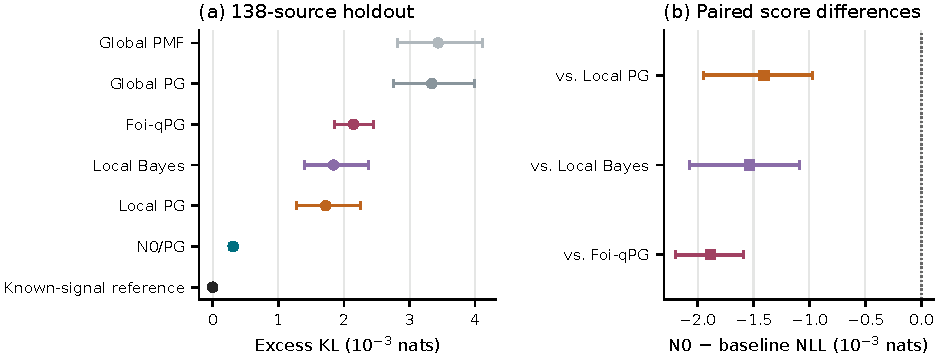
\includegraphics[width=\textwidth]{f03_holdout.pdf}
\caption{留出测试的条件分布精度。（a）平均超额 KL 及 95\% 源图 bootstrap 区间。（b）成对 NLL 差及 95\% 区间；负值有利于 N0。主要 97.5\% 比较区间见正文。}
\label{fig:holdout}
\end{figure*}

\subsection{信号与邻域结构的影响}\label{sec:regions}
空间估计的收益随信号水平和邻域结构而变化。亮边附近的零码与均匀暗区内的零码，在潜在信号和可见邻域信息上均有区别。因此，我们考察超额 KL 与信号强度、局部变化、梯度距离及观测零码比例的关系（图~\ref{fig:spatial}）；分箱定义见补充材料第~\ref{sec:regionaldefinitions} 节。

\subsubsection{信号水平}
近黑条件分布主要由校准读噪的负尾决定，不同信号估计产生的分布差异较小。相应地，N0 相对 Local Bayes 的平均超额 KL 差在 $s<0.25$ DN 时为 $-0.000087$ nats，而在 $8\leq s<16$ DN 时扩大至 $-0.002887$ nats。Foi-qPG 在 2 DN 以下的平均误差较低，N0 则在 4 DN 以上较低（图~\ref{fig:spatial}(a)）。

\subsubsection{邻域变化}
邻域结构也与误差差距有关。N0 相对 Local Bayes 的 KL 差在 $t<0.025$ 时为 $-0.000358$ nats，在 $t\geq0.8$ 时为 $-0.004467$ nats；两组的候选位置数分别为 379,366 和 98,229，对应源图数分别为 115 和 106。梯度位置的差值为 $-0.002200$ nats，距梯度至少 16 个打包像素时则为 $-0.000330$ nats。

观测到的零码比例提供了另一个视角：$z<0.1$ 时，N0 相对 Local Bayes 的 KL 差为 $-0.008058$ nats（17,450 个候选位置）；$0.5\leq z<0.75$ 时为 $-0.000226$ nats（498,135 个位置）。当删失位置周围大多是正码时，差距最大。信号强度和邻域变化具有相关性，因此第~\ref{sec:gradientcontrol} 节进一步在源图、CFA 和信号分箱内比较梯度差异。

\begin{figure*}[t]
\centering
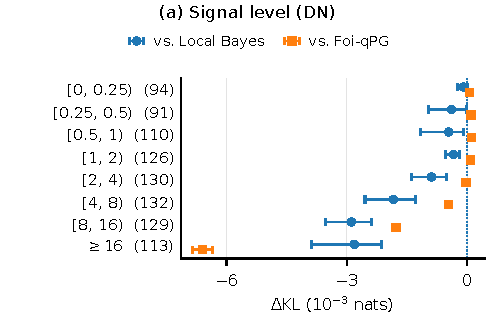
\includegraphics[width=0.493\textwidth]{f10a_holdout_signal.pdf}\hfill
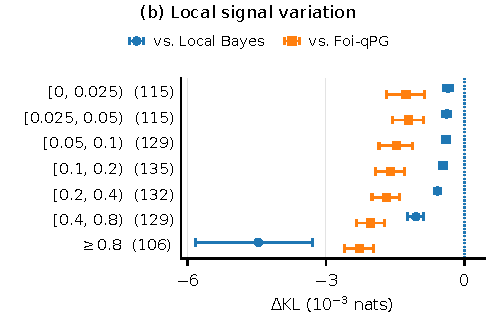
\includegraphics[width=0.493\textwidth]{f10b_holdout_variation.pdf}\\[1pt]
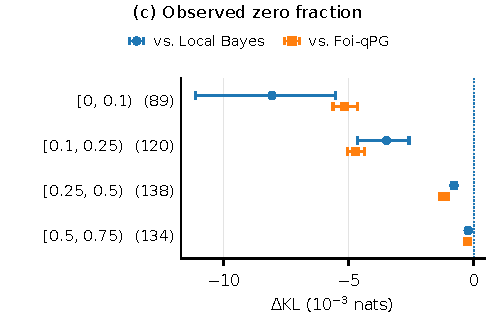
\includegraphics[width=0.493\textwidth]{f10c_holdout_zeros.pdf}\hfill
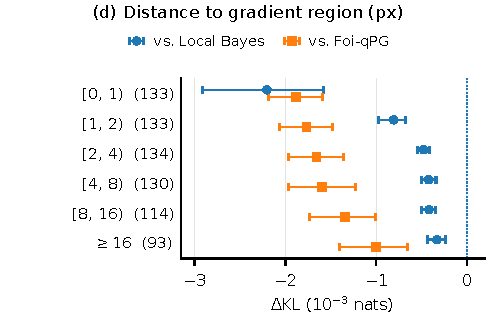
\includegraphics[width=0.493\textwidth]{f10d_holdout_gradient.pdf}
\caption{留出测试的区域误差差异，使用 256 像素上下文。点和误差条分别表示 N0 减 Local Bayes（圆形）或 Foi-qPG（方形）的超额 KL 差及 95\% 源图 bootstrap 区间；负值表示 N0 误差较低，括号内为源图数。（a）、（b）、（d）的信号和梯度特征来自模拟信号，（c）的零码比例来自输入 RAW。分组定义与计数见补充材料第~\ref{sec:regionaldefinitions} 节。}
\label{fig:spatial}
\end{figure*}

\subsection{空间信息的作用}
\subsubsection{跨 CFA 信息}
局部估计器也能联合利用四个 CFA 相位，而不构造多尺度信号场。在 32 幅开发源图的 32,462 个共同位置上，Joint-CFA Bayes、同 CFA Local PG 与 N0 的超额 KL 分别为 0.001790969、0.001952344 和 0.000376673（补充表~\ref{tab:joint}）。这一结果表明 N0 优于该局部构造，但二者除 CFA 信息外还存在空间上下文和先验容量的差别。

\subsubsection{位置分配}
为区分预测分布的整体组成与空间位置，我们在各开发源图及 CFA 相位内部置换预测信号，保持校准参数和预测概率律的集合不变。

这一改变就使 32 幅源图的超额 KL 从 0.0003719 升至 0.0026373（原位置减置换结果为 $-0.0022654$，95\% 区间 $[-0.0034895,-0.0012476]$）。这表明空间位置本身携带信息：预测分布的集合相同，分配给不同像素后仍会得到不同的评分。

\subsubsection{绝对误差与信号匹配对比}\label{sec:gradientcontrol}
两种估计器在高梯度区域的误差都增大，但 Local PG 增幅更大。在 32 幅开发源图中，低梯度组 N0／Local PG 的超额 KL 为 $0.000191/0.000791$，高梯度组则为 $0.000442/0.002109$。逐源图计算的配对 KL 差（N0 减 Local PG）从低梯度组到高梯度组变化量的均值为 $-0.001066$ nats（中位数 $-0.000102$，32 幅中有 23 幅小于零）。在同源、同 CFA 和信号分箱内进一步匹配，27 幅源图上的平均差仍为 $-0.000268$ nats；详细规则与 NLL 结果见补充材料第 IV 节。

\subsection{校准与模型失配}
N0 的 90\% 等尾整数区间覆盖留出码的 91.817\%，已知信号参考为 91.853\%。离散整数区间的实际概率质量可能高于标称值，因此补充表~\ref{tab:coverage} 还给出了按预测质量评估的四档覆盖率。





我们还考察了噪声假设改变后的表现。在扰动读噪或加入未建模行、列偏移的六种开发集设置下，N0 的平均 NLL 和 CRPS 均低于 Local PG；各差值与不确定性见补充图~\ref{fig:pairedstress}。

\subsection{真实传感器读出的条件分布}
两次 2400 万像素曝光 P2654748 和 P2654749 保留了标称黑电平以下的有符号传感器码。依据独立暗帧得到的逐相位整数平移，构造隐藏读出 $V$；两种方法均接收截零后的 $Y=\max(V,0)$。坐标变换与剩余小数偏移见补充材料第 V 节。

每次曝光取六个固定区域，R/$G_1$/$G_2$ 的主要评分集合分别包含 12,652 和 19,200 个删失位置。B 相位仍参与网络输入及抽样 Bayer 输出，但由于传感器统计不同，其真实数据评分仅作诊断。此处局部估计器使用 $3\times3$ 的同 CFA 邻域。

\begin{table}[t]
\centering\footnotesize
\setlength{\tabcolsep}{3pt}
\caption{真实有符号读数案例研究。每次曝光使用共享的 R/$G_1$/$G_2$ 候选项和固定真实数据方案。NLL 单位为每候选项 nats，CRPS 单位为 DN；数值越低越好。}
\label{tab:real}
\begin{tabular}{@{}lrrrr@{}}
\toprule
& \multicolumn{2}{c}{P2654748} & \multicolumn{2}{c}{P2654749}\\
\cmidrule(lr){2-3}\cmidrule(l){4-5}
方法 & NLL & CRPS & NLL & CRPS\\
\midrule
Global PMF & 3.980276 & 8.289612 & 4.005568 & 8.347404\\
Global PG & 3.979631 & 8.283446 & 4.004966 & 8.341612\\
Local PG & 3.975846 & 8.248081 & 4.004176 & 8.331820\\
Local Bayes & 3.978475 & 8.273926 & 4.006270 & 8.352316\\
Foi-qPG & 3.979516 & 8.283580 & 4.006041 & 8.350880\\
\textbf{N0/PG} & \textbf{3.974503} & \textbf{8.237064} & \textbf{4.003213} & \textbf{8.322619}\\
\bottomrule
\end{tabular}
\end{table}

在 P2654748 和 P2654749 中，N0 相对 Local PG 的 NLL 分别改善 0.001342 和 0.000964 nats，CRPS 分别改善 0.011017 和 0.009200 DN。第一次曝光中，N0 在六个 ROI 中的五个具有更低 NLL；第二次曝光中为六个中的两个。逐 ROI 结果见补充材料第~\ref{sec:realcode} 节及其对应数据。

校准 PG 模型明显低估了真实读出的极深负尾。在 31,852 个候选位置中，$V\leq-128$、$V\leq-256$、$V\leq-305$ DN 的观测次数分别为 122、21、13，而预测次数分别为 $9.01\times10^{-3}$、$3.76\times10^{-20}$、$8.63\times10^{-30}$。排除深尾事件或重复坐标后，N0 相对 Local PG 的配对 NLL 优势仍然保持（补充表~\ref{tab:real_robust}）。



\subsection{对去马赛克与颜色的影响}\label{sec:downstream}
\subsubsection{真实曝光的去马赛克统计}
为观察补全如何影响常规成像处理，我们使用同一个 AHD 实现对保留的有符号参考、截零版本、N0 样本及 Local PG 样本去马赛克。共同的数字基座值使负读出能够以 LibRaw 的无符号格式表示，并在颜色处理前从线性相机 RGB 中扣除。

对每个区域的 32 个条件样本分别去马赛克并计算空间统计量，再对这些逐次统计量取平均。在 P2654748 最暗区域中，钳位使线性 G 均值从 9.003 增至 16.322 DN；N0 和 Local PG 分别将其恢复至 8.621 和 8.602 DN。$R-G$ 的空间标准差经钳位从 25.986 降至 18.635 DN，N0 和 Local PG 分别使其恢复至 25.157 和 25.256 DN。因此，条件抽样恢复了删失所消除的大部分暗部起伏，两种估计器的统计结果相近。两次曝光的结果见补充表~\ref{tab:ahd}。

处理顺序示意与 AHD 实现细节见补充材料第 V 节及 \href{visual_zh.pdf}{补充图像 A}。

\subsubsection{合成场景中基于干净参考的暗部颜色误差}
另一项开发集实验进一步考察负码补全对渲染后暗部颜色的影响。八幅自然场景和四个程序化模板经过 AHD、四倍有符号域平均，以及固定的白平衡、颜色转换和曝光缩放。以量化干净信号为参考，在线性显示 RGB 中计算块均值色度向量 $(R-G,B-G)$ 的平方误差（补充材料第~\ref{sec:cleanendpoint} 节）。

在自然场景中，直接截零使颜色误差由有符号读出的 0.125006 升至 1.257683。条件抽样使误差降至接近有符号参考的水平：N0 为 0.122891，Local PG 为 0.126031。N0 减 Local 的差值为 $-0.00314$（95\% 源图 bootstrap 区间 $[-0.00614,-0.00084]$），在八幅自然开发源图上的相对降幅为 2.49\%。改用量化条件均值时，两者分别为 0.102618 和 0.105440（表~\ref{tab:cleanendpoint}）；四个程序化场景另行报告。

\begin{table}[t]
\centering\small
\setlength{\tabcolsep}{4pt}
\caption{八幅自然开发源图的暗部颜色误差与干净 RAW MSE，采用源图等权汇总。颜色误差为经曝光缩放的线性显示 RGB 中块均值 $(R-G,B-G)$ 的平方误差；RAW MSE 以 $Q(s)$ 为参考，单位为 DN$^2$。原始有符号输入是未删失的含噪读出。两项指标均为数值越低越好。}
\label{tab:cleanendpoint}
\begin{tabular}{@{}lrr@{}}
\toprule
RAW 输入 & 暗部颜色误差 & RAW MSE\\
\midrule
原始有符号 & 0.125006 & 1157.747\\
直接钳位 & 1.257683 & \textbf{866.698}\\
Local PG 抽样 & 0.126031 & 1157.244\\
N0/PG 抽样 & \textbf{0.122891} & 1159.305\\
Local PG 均值-$Q$ & 0.105440 & 1077.675\\
N0/PG 均值-$Q$ & \textbf{0.102618} & 1076.179\\
\bottomrule
\end{tabular}
\end{table}

两类指标的排序取决于评价目标。对于非负干净参考 $c=Q(s)$ 和任意允许的填充值 $k\leq0$，有 $(k-c)^2-c^2=k^2-2kc\geq0$。因此，在正码保持不变的约束下，零填充使干净 RAW 的逐像素 MSE 最小；但它改变了暗部均值，在表~\ref{tab:cleanendpoint} 中产生最大的块颜色误差。对于本次固定渲染实验，量化条件均值的颜色误差最低。

\subsection{运行时间与全分辨率推理}\label{sec:runtime}
在 RTX 3090 Ti 上，N0/PG 对 2400 万像素读出完成补全需要 27.3901 s，Local PG 为 205.1503 s；两者的 CUDA 峰值已分配显存分别为 750.69 和 94.84 MiB。两者使用不同数值后端，补充表~\ref{tab:runtime} 列出实测实现条件。

全分辨率推理采用相位对齐的重叠分块（补充材料第 VI 节）。对于固定条件概率律，坐标索引抽样不受分块顺序影响（补充材料第 III 节）。

\section{讨论}
留出实验将条件读出分布的精度与预测所处的图像位置联系起来。信号变化明显时，局部常值模型的误差较大，多尺度估计的优势也更突出。在保持预测集合不变的条件下置换其位置，超额 KL 仍会增大。这些结果表明，预测分布的空间分配是条件补全精度的重要来源。

分布评分反映条件读出概率律的估计精度，下游图像统计还受到去马赛克和颜色处理的影响。匹配模型下的合成实验使用已知信号 PG 条件律衡量估计误差。在真实曝光中，共享的噪声模型严重低估罕见极负码，但 N0 仍具有较小的配对似然优势。两类抽样方法都恢复了部分去马赛克暗部起伏；固定渲染开发实验进一步显示，零填充虽能最小化干净 RAW MSE，却可能扭曲暗部颜色。

本研究的合成实验刻画了单一高增益校准参数组下的估计精度。真实读出进一步表明，整体评分的改善可以与罕见极负码的严重失配同时存在；其他传感器模式仍需分别考察尾部校准。

\section{结论}
下限删失 RAW 图像中的一个零码可能对应多个有符号整数读出。N0/PG 利用邻近 Bayer 测量估计各位置的离散条件律，仅在删失位置抽样，保留所有正码。在 138 幅留出源图上，该空间估计优于所比较的局部与变换域方法。真实有符号读出和固定渲染开发实验进一步展示了缺失负码对暗部统计与颜色的影响。

\section*{可复现性声明}
随附仓库提供表格评分、源图标识、颜色评价记录、训练所得参数及推理和评价代码。推理示例已在隔离环境验证。发布清单记录所分发文件的 SHA-256。原创代码和模型权重采用 MIT 许可；原创论文图件与数值结果采用 CC BY 4.0。第三方材料保留各自许可。

\section*{致谢}
OpenAI Codex 和 Kimi 辅助了程序实现、稿件起草和语言编辑。

\begin{thebibliography}{10}
\fontsize{7.8}{8.1}\selectfont
\setlength{\itemsep}{0pt}
\bibitem{foi2008} A. Foi, M. Trimeche, V. Katkovnik, and K. Egiazarian, ``Practical Poissonian--Gaussian noise modeling and fitting for single-image raw-data,'' \emph{IEEE Transactions on Image Processing}, vol. 17, no. 10, pp. 1737--1754, 2008. doi: 10.1109/TIP.2008.2001399.
\bibitem{foi2009} A. Foi, ``Clipped noisy images: Heteroskedastic modeling and practical denoising,'' \emph{Signal Processing}, vol. 89, no. 12, pp. 2609--2629, 2009. doi: 10.1016/j.sigpro.2009.04.035.
\bibitem{mathworksISP} MathWorks, ``End-to-End Implementation of a Digital Camera Processing Pipeline,'' Image Processing Toolbox documentation, accessed 28 October 2026. \url{https://ww2.mathworks.cn/help/images/end-to-end-implementation-of-digital-camera-processing-pipeline.html}
\bibitem{librawD5300} LibRaw technical support, ``Nikon NEF RAW Data Minimum Value Clamp: D5300 Code-Floor Investigation,'' 2018. \url{https://www.libraw.org/node/2362}
\bibitem{claffReadNoise} B. Claff, ``Read Noise: The Effect of Black Clipping in Nikon D70 Dark Frames,'' Photons to Photos, prepared 25 November 2007, accessed 28 October 2026. \url{https://photonstophotos.net/GeneralTopics/Sensors_&_Raw/Read_Noise.htm}
\bibitem{aim2025Video} A. Yakovenko, G. Chakvetadze, I. Khrapov, M. Zhelezov, D. Vatolin, R. Timofte, et al., ``AIM 2025 Low-light RAW Video Denoising Challenge: Dataset, Methods and Results,'' in \emph{Proc. IEEE/CVF ICCV Workshops}, pp. 5703--5713, 2025. \url{https://arxiv.org/html/2508.16830}
\bibitem{sonyAIM2025} Sony Research, ``AIM 2025 Challenge on Low-Light Real-World RAW Image Denoising Using Synthetic Data: Official Starter Kit,'' 2025. \url{https://github.com/SonyResearch/AIM2025_Denoise_Challenge/blob/main/README.md}
\bibitem{nafnet} L. Chen, X. Chu, X. Zhang, and J. Sun, ``Simple baselines for image restoration,'' in \emph{European Conference on Computer Vision}, 2022, pp. 17--33. doi: 10.1007/978-3-031-20071-7\_2.
\bibitem{oneill2024} E. O'Neill, ``Type I Tobit Bayesian additive regression trees for censored outcome regression,'' \emph{Statistics and Computing}, vol. 34, art. 123, 2024. doi: 10.1007/s11222-024-10434-4.
\bibitem{kodgirwar2024} S. Kodgirwar, L. Loetgering, C. Liu, A. Joseph, L. Licht, D. S. Penagos Molina, W. Eschen, J. Rothhardt, and M. Habeck, ``Bayesian multi-exposure image fusion for robust high dynamic range ptychography,'' \emph{Optics Express}, vol. 32, no. 16, pp. 28090--28099, 2024. doi: 10.1364/OE.524284.
\bibitem{wei2020} K. Wei, Y. Fu, J. Yang, and H. Huang, ``A physics-based noise formation model for extreme low-light raw denoising,'' in \emph{IEEE/CVF Conference on Computer Vision and Pattern Recognition}, 2020, pp. 2758--2767. doi: 10.1109/CVPR42600.2020.00283.
\bibitem{zhang2021} Y. Zhang, H. Qin, X. Wang, and H. Li, ``Rethinking noise synthesis and modeling in raw denoising,'' in \emph{Proceedings of the IEEE/CVF International Conference on Computer Vision}, 2021, pp. 4593--4601. doi: 10.1109/ICCV48922.2021.00455.
\bibitem{mohammadi2026} M. Mohammadi, S. Honari, S. Tsogkas, T. Aumentado-Armstrong, M. S. Brown, I. Mohomed, K. G. Derpanis, A. Levinshtein, and I. Gilitschenski, ``Why low-light cameras go color blind: Removing color bias in raw denoising,'' \emph{arXiv preprint arXiv:2607.11090}, 2026.
\bibitem{gilton2021} D. Gilton, G. Ongie, and R. Willett, ``Deep equilibrium architectures for inverse problems in imaging,'' \emph{IEEE Transactions on Computational Imaging}, vol. 7, pp. 1123--1133, 2021. doi: 10.1109/TCI.2021.3118944.
\bibitem{goujon2023} A. Goujon, S. Neumayer, P. Bohra, S. Ducotterd, and M. Unser, ``A neural-network-based convex regularizer for inverse problems,'' \emph{IEEE Transactions on Computational Imaging}, vol. 9, pp. 781--795, 2023. doi: 10.1109/TCI.2023.3306100.
\bibitem{bohra2022} P. Bohra, T.-a. Pham, J. Dong, and M. Unser, ``Bayesian inversion for nonlinear imaging models using deep generative priors,'' \emph{IEEE Transactions on Computational Imaging}, vol. 8, pp. 1237--1249, 2022. doi: 10.1109/TCI.2023.3236155.
\bibitem{gnanasambandam2024} A. Gnanasambandam, Y. Sanghvi, and S. H. Chan, ``The secrets of non-blind Poisson deconvolution,'' \emph{IEEE Transactions on Computational Imaging}, vol. 10, pp. 343--356, 2024. doi: 10.1109/TCI.2024.3369414.
\bibitem{gneiting2007} T. Gneiting and A. E. Raftery, ``Strictly proper scoring rules, prediction, and estimation,'' \emph{Journal of the American Statistical Association}, vol. 102, no. 477, pp. 359--378, 2007. doi: 10.1198/016214506000001437.
\bibitem{gharbi2016} M. Gharbi, G. Chaurasia, S. Paris, and F. Durand, ``Deep joint demosaicking and denoising,'' \emph{ACM Transactions on Graphics}, vol. 35, no. 6, pp. 191:1--191:12, 2016. doi: 10.1145/2980179.2982399.
\bibitem{hirakawa2005} K. Hirakawa and T. W. Parks, ``Adaptive homogeneity-directed demosaicing algorithm,'' \emph{IEEE Transactions on Image Processing}, vol. 14, no. 3, pp. 360--369, 2005. doi: 10.1109/TIP.2004.838691.
\bibitem{libraw} LibRaw contributors, ``LibRaw 0.22.1, pinned source revision b860248a89d9082b8e0a1e202e516f46af9adb29,'' software source, accessed 27 October 2026. \url{https://github.com/LibRaw/LibRaw/tree/b860248a89d9082b8e0a1e202e516f46af9adb29}
\bibitem{jot} JOT measurement resource, ``Photon-transfer measurement record: Panasonic S5 II, ISO12800, mechanical shutter,'' archived measurement resource, 2026. \url{https://y-g-jiang.github.io/JOT.html}
\bibitem{div2k} E. Agustsson and R. Timofte, ``NTIRE 2017 challenge on single image super-resolution: Dataset and study,'' in \emph{IEEE Conference on Computer Vision and Pattern Recognition Workshops}, 2017, pp. 126--135. doi: 10.1109/CVPRW.2017.150.
\bibitem{bsds500} P. Arbeláez, M. Maire, C. Fowlkes, and J. Malik, ``Contour detection and hierarchical image segmentation,'' \emph{IEEE Transactions on Pattern Analysis and Machine Intelligence}, vol. 33, no. 5, pp. 898--916, 2011. doi: 10.1109/TPAMI.2010.161.
\bibitem{bm3d} K. Dabov, A. Foi, V. Katkovnik, and K. Egiazarian, ``Image denoising by sparse 3-D transform-domain collaborative filtering,'' \emph{IEEE Transactions on Image Processing}, vol. 16, no. 8, pp. 2080--2095, 2007. doi: 10.1109/TIP.2007.901238.
\end{thebibliography}
\end{document}
